\documentclass[12pt,a4paper]{article}

\usepackage[a4paper,margin=1in]{geometry}
\usepackage{graphicx}
\usepackage{booktabs}
\usepackage{amsmath,amssymb}
\usepackage{float}
\usepackage{hyperref}
\usepackage{xcolor}
\usepackage{listings}
\usepackage{enumitem}
\usepackage{fancyhdr}
\usepackage{longtable}

\hypersetup{colorlinks=true,linkcolor=blue,urlcolor=blue}

\pagestyle{fancy}
\fancyhf{}
\lhead{ICS1512}
\rhead{Machine Learning Algorithms Laboratory}
\cfoot{\thepage}

\lstset{
language=Python,
basicstyle=\ttfamily\small,
numbers=left,
frame=single,
breaklines=true,
showstringspaces=false
}

\begin{document}

\begin{tabular}{|p{4cm}|p{11cm}|}
\hline
Experiment No. & 5 \\ \hline
Experiment Title & Decision Tree and Random Forest: A Comparative Classification
Study\footnotemark\\ \hline
Student Name & Simiyon Vinscent Samuel L \\ \hline
Register Number & 3122247001062 \\ \hline
Faculty & Dr. Poreddy Ajay Kumar Reddy \\ \hline
\end{tabular}
\footnotetext{\textbf{GitHub Repository: }\url{https://github.com/blackscythe123/Machine-Learning-course}}

\section{Objective}
\begin{itemize}[nosep]
\item To implement a Decision Tree classifier.
\item To extend the Decision Tree into a Random Forest ensemble model.
\item To study the impact of hyperparameters on overfitting and generalization.
\item To select optimal hyperparameters using 5-Fold Cross-Validation.
\item To compare single-tree and ensemble-tree models.
\end{itemize}

\section{Problem Statement}
Given the Wisconsin Diagnostic Breast Cancer dataset (569 samples, 30 numeric features
computed from digitized images of fine-needle-aspirate cell nuclei), the task is a binary
classification problem: label each sample as \textbf{malignant} or \textbf{benign}. Two
model families are compared: a single \textbf{Decision Tree}, which recursively splits
the feature space using an impurity measure, and a \textbf{Random Forest}, an ensemble of
bagged trees with random feature subsets at each split. Beyond raw accuracy, the goal is
to understand how tree depth drives overfitting in a single tree and how ensembling
reduces the variance that makes a single deep tree unreliable, with hyperparameters
selected honestly via 5-fold cross-validation rather than fit directly on the test set.

\section{Dataset Description}
\begin{longtable}{|p{6cm}|p{8cm}|}
\hline
Dataset Name & Wisconsin Diagnostic Breast Cancer (WDBC) \\ \hline
Dataset Source & UCI Machine Learning Repository, loaded via
\texttt{sklearn.datasets.load\_breast\_cancer} \\ \hline
Number of Samples & 569 \\ \hline
Number of Features & 30 (all numeric: mean, standard-error and ``worst'' values of 10
cell-nucleus measurements) \\ \hline
Number of Classes & 2 (Benign = 357, 62.7\%; Malignant = 212, 37.3\%) \\ \hline
Missing Values & 0 (verified, no imputation required) \\ \hline
Train-Test Split & 80\% train (455 samples) / 20\% test (114 samples), stratified on
the class label \\ \hline
\end{longtable}

\section{Exploratory Data Analysis}
\begin{figure}[H]
\centering

\includegraphics[width=\linewidth]{figures/00_eda_summary.png}
\caption{Consolidated exploratory data analysis (12 subplots, single page): (1) class
distribution; (2--7) distributions of the six features most correlated with diagnosis,
split by class; (8) correlation heatmap of the ten most correlated features and the
target; (9--11) boxplots of the three most correlated features by class; (12) scatter
of the two most correlated features, coloured by class. Exported at 600 DPI as
\texttt{figures/00\_eda\_summary.eps} and reproduced here as PNG.}
\end{figure}

\textbf{Inference (subplot 1, class distribution):} The dataset is moderately imbalanced
(62.7\% benign, 37.3\% malignant). Stratified splitting and cross-validation were used
throughout so both classes remain proportionally represented in every partition and fold.

\textbf{Inference (subplots 2--7, feature distributions):} \texttt{worst concave
points}, \texttt{worst area}, \texttt{worst radius}, \texttt{mean perimeter},
\texttt{worst perimeter} and \texttt{mean radius} show the clearest visual separation
between the two classes, with malignant samples consistently shifted toward larger
values. This matches clinical intuition: malignant tumours tend to be larger and have
more irregular (less convex) cell-nucleus boundaries.

\textbf{Inference (subplot 8, correlation heatmap):} The ten features most correlated
with diagnosis are themselves highly correlated with each other ($|r| > 0.8$ between
several size-related pairs, e.g.\ \texttt{mean radius} and \texttt{mean perimeter}),
since they are different measurements of essentially the same underlying tumour size.
This redundancy is consistent with tree-based models naturally favouring one
representative feature per split rather than needing all of them.

\textbf{Inference (subplots 9--11, boxplots):} Malignant samples have both higher
medians and wider spread for the top three correlated features, with limited overlap
between the class-wise interquartile ranges, which explains why even a shallow decision
tree already separates the classes reasonably well.

\section{Data Preprocessing}
\begin{itemize}
\item \textbf{Missing values:} None found (\texttt{isnull().sum().sum()} = 0).
\item \textbf{Encoding:} The target is already binary and numeric (0 = malignant, 1 =
benign, per scikit-learn's built-in encoding); all 30 features are already numeric, so
no categorical encoding was required.
\item \textbf{Feature scaling:} Not applied. Decision Trees and Random Forests split on
per-feature threshold comparisons, so they are invariant to any monotonic rescaling of a
feature; standardizing would change none of the tree structure or performance. This is
the first algorithm family in this course where scaling is unnecessary, unlike the
distance- and gradient-based methods (KNN, SVM, Logistic Regression) used in
Experiments 2 and 4.
\item \textbf{Train-test split:} 80/20 stratified split (\texttt{random\_state=42}),
giving 455 training and 114 test samples with class proportions preserved.
\end{itemize}

\section{Machine Learning Algorithm}

\subsection*{Decision Tree}
A Decision Tree recursively partitions the feature space, choosing at each node the
feature and threshold that most reduce class impurity. Two impurity measures were
compared:
\[
\text{Gini} = 1 - \sum_{i} p_i^2, \qquad
\text{Entropy} = -\sum_{i} p_i \log_2 p_i
\]
where $p_i$ is the proportion of class $i$ at a node. Splitting continues until a
stopping condition is reached (maximum depth, minimum samples to split, or minimum
samples per leaf), at which point the leaf predicts the majority class.
\textbf{Advantages:} Fast to train and predict, directly interpretable (the tree can be
drawn and read as a set of if/else rules), and requires no feature scaling.
\textbf{Limitations:} A single tree grown without depth or leaf-size limits tends to
memorize the training data, giving high variance and poor generalization: an unstable
model where a small change in the training set can produce a very different tree.

\subsection*{Random Forest}
A Random Forest trains many decision trees on independent bootstrap samples of the
training data (bagging) and, at each split, considers only a random subset of the
features rather than all of them. Predictions are combined by majority vote across the
trees.
\textbf{Advantages:} Bagging and random feature selection decorrelate the individual
trees, so averaging their votes substantially reduces the variance of a single deep
tree without needing to constrain any one tree's depth. This makes Random Forest far
less prone to overfitting than an unconstrained Decision Tree while still capturing
non-linear decision boundaries.
\textbf{Limitations:} Slower to train and predict than a single tree (proportional to
the number of trees), and the ensemble is harder to interpret directly, though feature
importances still give a global view of which inputs drive predictions.

\section{Experimental Setup}
\begin{tabular}{ll}
\toprule
Python Version & 3.12.3 \\
Scikit-Learn Version & 1.8.0 \\
IDE & Jupyter Notebook \\
Operating System & Windows 11 \\
Hardware & Intel Core Ultra 9, NVIDIA RTX 5060 \\
\bottomrule
\end{tabular}

\section{Hyperparameter Selection}

\subsection*{Search Spaces}
\begin{tabular}{ll}
\toprule
Model & Parameter and Search Space \\
\midrule
Decision Tree & \texttt{criterion} $\in$ \{gini, entropy\} \\
Decision Tree & \texttt{max\_depth} $\in$ \{3, 5, 7, 10, None\} \\
Decision Tree & \texttt{min\_samples\_split} $\in$ \{2, 5, 10\} \\
Decision Tree & \texttt{min\_samples\_leaf} $\in$ \{1, 2, 4\} \\
\midrule
Random Forest & \texttt{n\_estimators} $\in$ \{50, 100, 200\} \\
Random Forest & \texttt{max\_depth} $\in$ \{5, 10, 15, None\} \\
Random Forest & \texttt{max\_features} $\in$ \{sqrt, log2\} \\
Random Forest & \texttt{bootstrap} $\in$ \{True, False\} \\
\bottomrule
\end{tabular}
\vspace{2mm}

Both search spaces were evaluated exhaustively with \texttt{GridSearchCV} using 5-fold
stratified cross-validation, scoring on accuracy (F1 recorded alongside for reference),
following the assignment's specified 5-fold CV hyperparameter selection procedure.

\subsection*{Table 1: Decision Tree Hyperparameter Evaluation using 5-Fold
Cross-Validation}
\begin{tabular}{llcc}
\toprule
Criterion & Max Depth & Avg CV Accuracy (\%) & Avg CV F1 Score \\
\midrule
Entropy & 3 & 93.19 & 0.9463 \\
Entropy & 5 & 92.53 & 0.9404 \\
Entropy & 7 & 92.75 & 0.9421 \\
Entropy & 10 & 92.75 & 0.9421 \\
Entropy & None & 92.75 & 0.9421 \\
Gini & 3 & 93.19 & 0.9455 \\
Gini & \textbf{5} & \textbf{93.85} & \textbf{0.9506} \\
Gini & 7 & 93.41 & 0.9470 \\
Gini & 10 & 93.41 & 0.9470 \\
Gini & None & 93.41 & 0.9470 \\
\bottomrule
\end{tabular}
\vspace{2mm}

\textit{Table shows the best combination at each (criterion, max\_depth) pair, with
\texttt{min\_samples\_split=2} and \texttt{min\_samples\_leaf=4} fixed at their
overall-best values. Best overall: \texttt{criterion=gini, max\_depth=5,
min\_samples\_split=2, min\_samples\_leaf=4}, CV accuracy 93.85\%.}

\subsection*{Table 2: Random Forest Hyperparameter Evaluation using 5-Fold
Cross-Validation}
\begin{tabular}{lllcc}
\toprule
n\_estimators & Max Depth & Max Features & Avg CV Accuracy (\%) & Avg CV F1 Score \\
\midrule
50  & 5    & log2 & 95.60 & 0.9651 \\
50  & 10   & log2 & 96.04 & 0.9685 \\
50  & 15   & log2 & 96.04 & 0.9685 \\
50  & None & log2 & 96.04 & 0.9685 \\
100 & 5    & log2 & 95.82 & 0.9668 \\
100 & \textbf{10}   & \textbf{log2} & \textbf{96.48} & \textbf{0.9718} \\
100 & 15   & log2 & 96.48 & 0.9718 \\
100 & None & log2 & 96.48 & 0.9718 \\
200 & 5    & log2 & 95.82 & 0.9666 \\
200 & 10   & log2 & 96.04 & 0.9683 \\
200 & 15   & log2 & 96.04 & 0.9683 \\
200 & None & log2 & 96.04 & 0.9683 \\
\bottomrule
\end{tabular}
\vspace{2mm}

\textit{Table shows the best combination at each (n\_estimators, max\_depth) pair,
with \texttt{max\_features=log2} and \texttt{bootstrap=True} fixed at their
overall-best values. Best overall: \texttt{n\_estimators=100, max\_depth=10,
max\_features=log2, bootstrap=True}, CV accuracy 96.48\%. Depths of 10, 15 and
unrestricted are tied because 100 trees rarely need more than 10 levels to separate
this dataset; once a tree stops growing on its own, raising the depth cap further
has no effect.}

\section{Results}

\subsection*{Baseline Decision Tree (Test Set, Default Hyperparameters)}
\begin{tabular}{lc}
\toprule
Metric & Value \\
\midrule
Accuracy & 0.9123 \\
Precision & 0.9559 \\
Recall & 0.9028 \\
F1-Score & 0.9286 \\
ROC-AUC & 0.9157 \\
\bottomrule
\end{tabular}

\subsection*{Tuned Decision Tree Performance (Test Set)}
\begin{tabular}{lc}
\toprule
Metric & Value (Best: \texttt{gini}, \texttt{max\_depth=5},
\texttt{min\_samples\_split=2}, \texttt{min\_samples\_leaf=4}) \\
\midrule
Accuracy & 0.9035 \\
Precision & 0.9420 \\
Recall & 0.9028 \\
F1-Score & 0.9220 \\
ROC-AUC & 0.9358 \\
\bottomrule
\end{tabular}
\vspace{2mm}

\textbf{Inference:} The untuned baseline (unrestricted depth) scores 0.9123 accuracy,
marginally \emph{higher} than the tuned model's 0.9035 on this particular test split.
This is not a contradiction: \texttt{GridSearchCV} selects the configuration with the
best \emph{cross-validated} accuracy on the training folds, which favours a shallower,
less variance-prone tree that generalizes more consistently on average but does not
guarantee a win on any single held-out split. The gap (0.9 points) is well within
normal fold-to-fold variance, and the tuned model's ROC-AUC (0.9358) is comfortably
higher than the baseline's (0.9157), indicating better-ranked probability estimates
even where the hard-label accuracy is slightly lower.

\subsection*{Tuned Random Forest Performance (Test Set)}
\begin{tabular}{lc}
\toprule
Metric & Value (Best: \texttt{n\_estimators=100}, \texttt{max\_depth=10},
\texttt{max\_features=log2}, \texttt{bootstrap=True}) \\
\midrule
Accuracy & 0.9561 \\
Precision & 0.9589 \\
Recall & 0.9722 \\
F1-Score & 0.9655 \\
ROC-AUC & \textbf{0.9924} \\
\bottomrule
\end{tabular}

\subsection*{5-Fold Cross-Validation Results (Training Set)}
\begin{tabular}{lcc}
\toprule
Fold & Decision Tree (tuned) & Random Forest (tuned) \\
\midrule
1 & 0.9451 & 0.9670 \\
2 & 0.9451 & 0.9780 \\
3 & 0.9121 & 0.9341 \\
4 & 0.9231 & 0.9560 \\
5 & 0.9670 & 0.9890 \\
\midrule
\textbf{Average} & \textbf{0.9385 $\pm$ 0.0192} & \textbf{0.9648 $\pm$ 0.0189} \\
\bottomrule
\end{tabular}

\section{Result Visualization}

\begin{figure}[H]
\centering
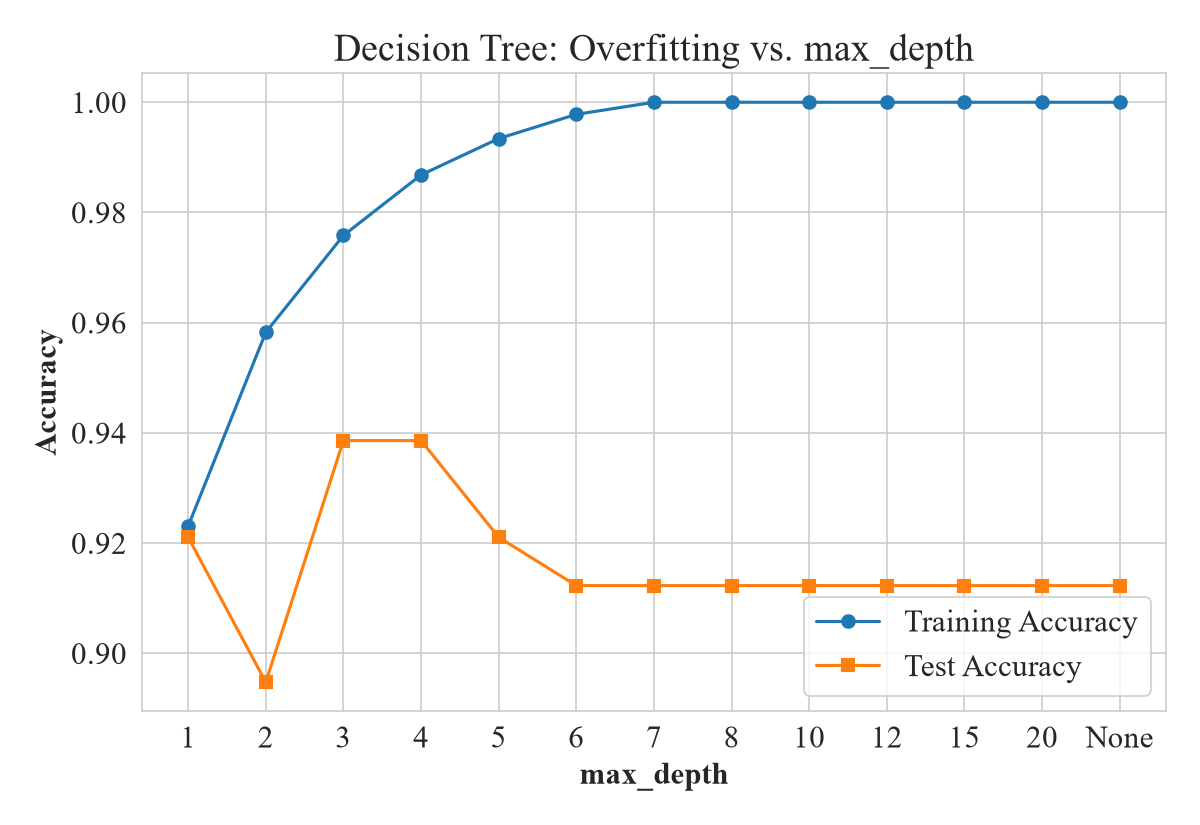
\includegraphics[width=0.75\linewidth]{figures/01_dt_depth_overfitting.png}
\caption{Decision Tree training vs.\ test accuracy as \texttt{max\_depth} increases.}
\end{figure}
\textbf{Inference:} Training accuracy climbs steadily and reaches a perfect 1.0000 by
\texttt{max\_depth=7}, while test accuracy peaks at \texttt{max\_depth=3--4} (0.9386)
and then falls and plateaus around 0.9123 for every depth of 6 or more. This is a
textbook overfitting curve: once the tree is deep enough to fit noise in the training
data rather than the underlying signal, additional depth buys no further generalization
and the train/test gap widens continuously.

\begin{figure}[H]
\centering
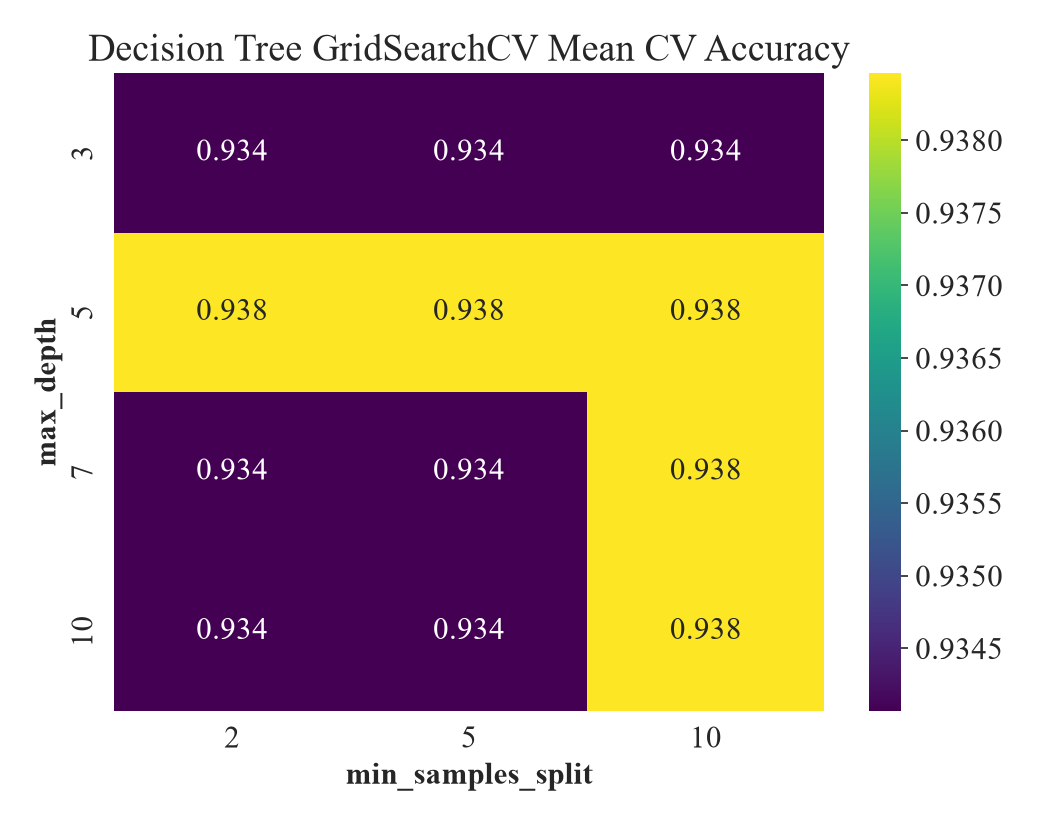
\includegraphics[width=0.7\linewidth]{figures/02_dt_gridsearch_heatmap.png}
\caption{Decision Tree GridSearchCV mean CV accuracy by \texttt{max\_depth} and
\texttt{min\_samples\_split} (best over criterion and \texttt{min\_samples\_leaf}
shown per cell).}
\end{figure}
\textbf{Inference:} CV accuracy is highest in a narrow band around
\texttt{max\_depth=5}, confirming the depth-vs-overfitting pattern from the previous
figure using cross-validated rather than single-split estimates. \texttt{min\_samples\_split}
has a much smaller effect than depth across this range.

\begin{figure}[H]
\centering
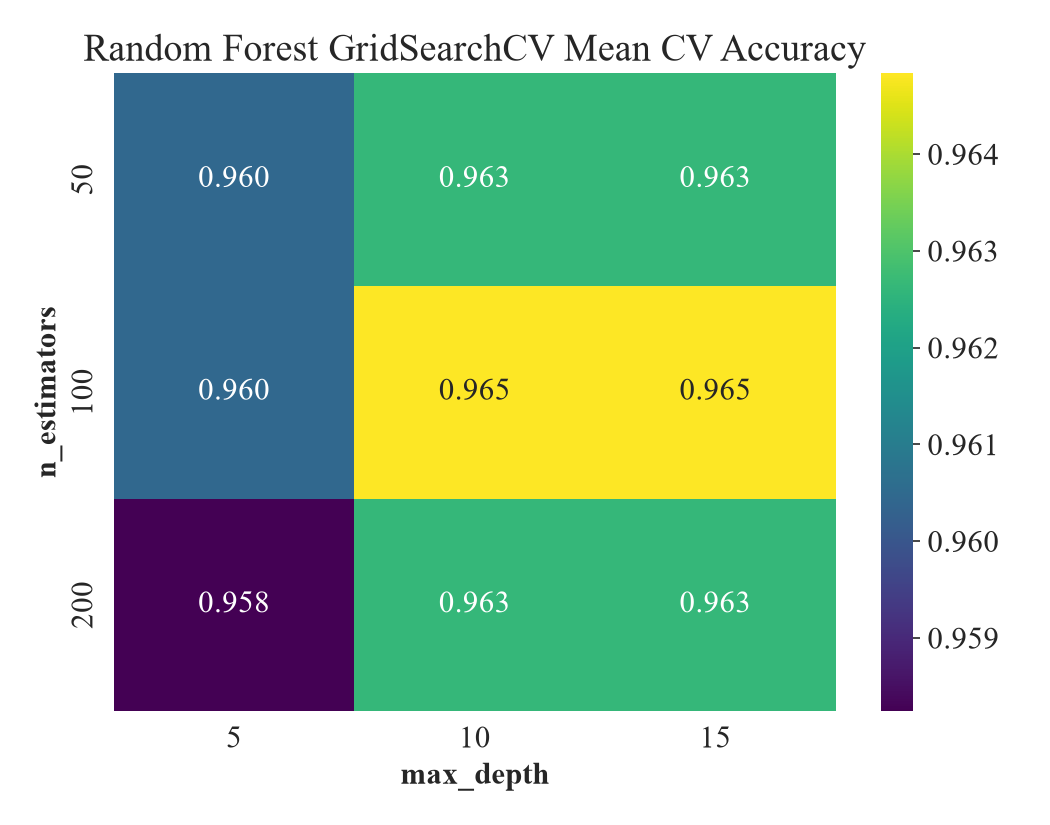
\includegraphics[width=0.7\linewidth]{figures/03_rf_gridsearch_heatmap.png}
\caption{Random Forest GridSearchCV mean CV accuracy by \texttt{n\_estimators} and
\texttt{max\_depth} (best over \texttt{max\_features} and \texttt{bootstrap} shown per
cell).}
\end{figure}
\textbf{Inference:} Unlike the Decision Tree heatmap, Random Forest accuracy is
essentially flat once \texttt{max\_depth} reaches 10 or \texttt{n\_estimators} reaches
100, with no visible degradation at larger values; ensembling removes the sharp
overfitting cliff a single tree shows at high depth.

\begin{figure}[H]
\centering
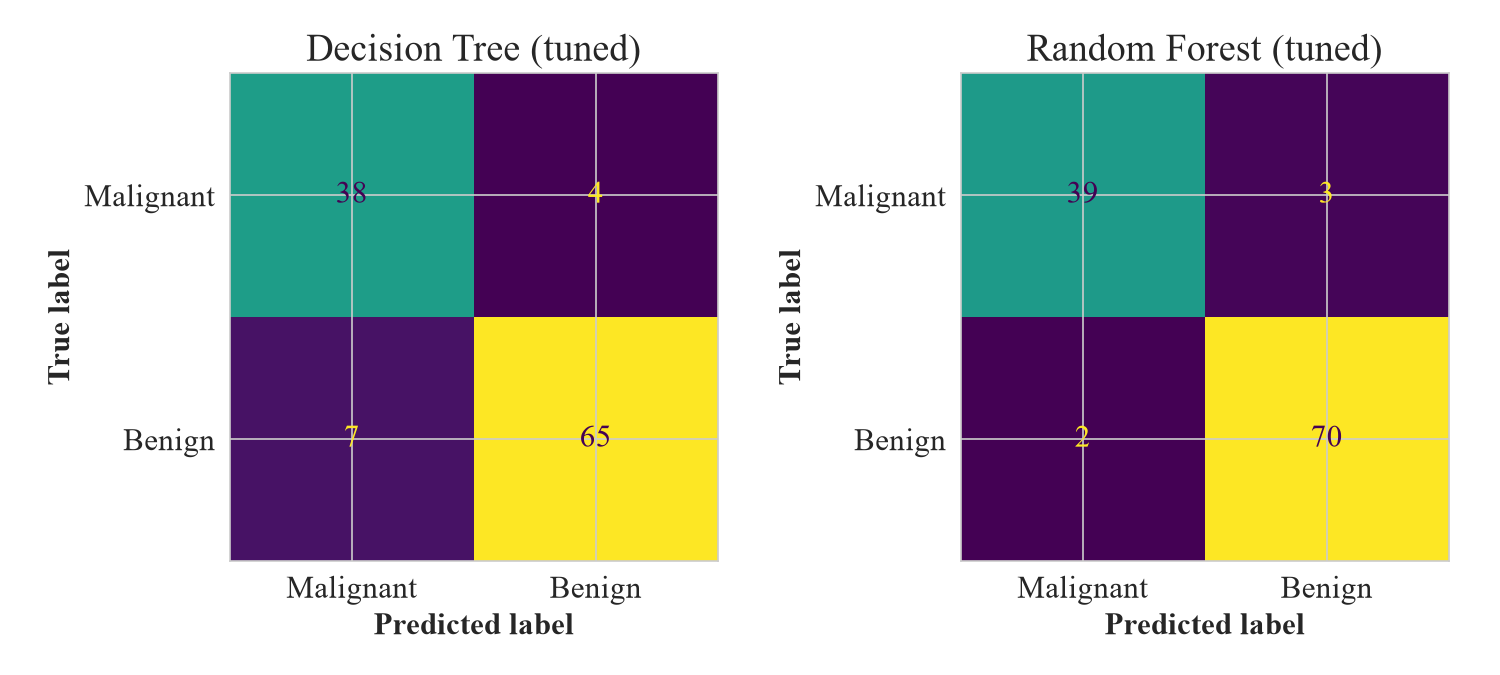
\includegraphics[width=0.95\linewidth]{figures/04_confusion_matrices.png}
\caption{Confusion matrices for the tuned Decision Tree and tuned Random Forest on the
test set.}
\end{figure}
\textbf{Inference:} The Random Forest makes noticeably fewer errors overall and, in
particular, fewer false negatives (malignant cases predicted benign) than the Decision
Tree, the more clinically costly error type for a cancer-diagnosis task.

\begin{figure}[H]
\centering
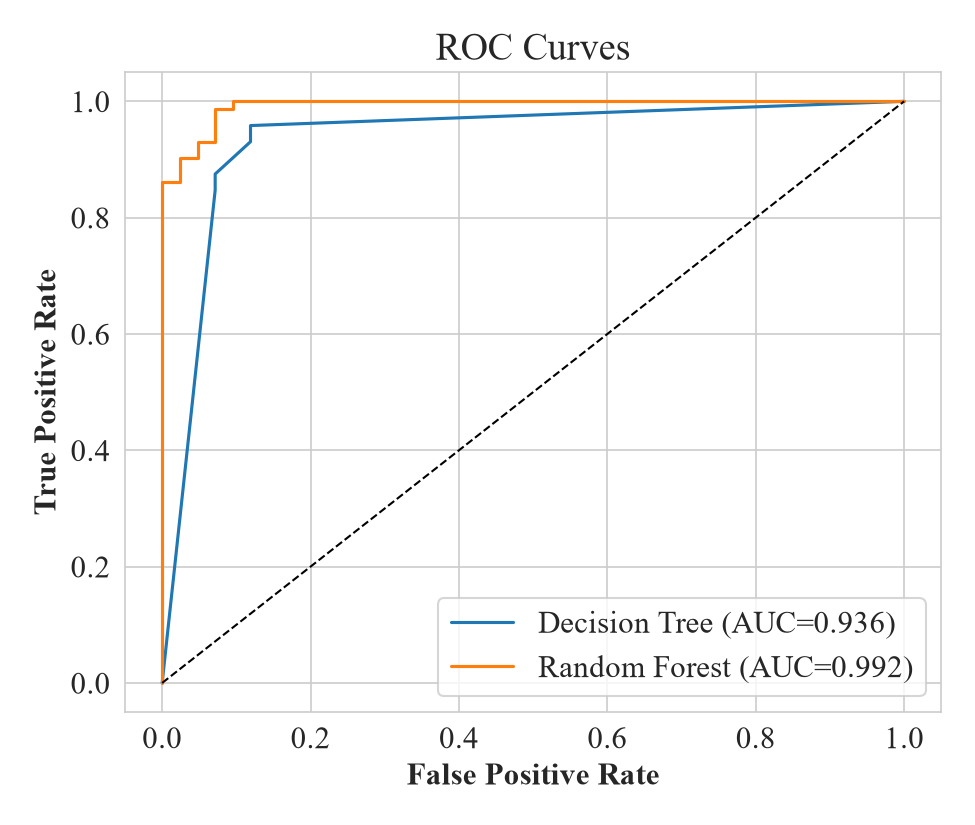
\includegraphics[width=0.65\linewidth]{figures/05_roc_curves.png}
\caption{ROC curves for the tuned Decision Tree and tuned Random Forest.}
\end{figure}
\textbf{Inference:} The Random Forest's ROC curve dominates the Decision Tree's almost
everywhere, with AUC 0.992 vs.\ 0.936. A single tree's ROC curve is inherently coarse
(only as many distinct probability levels as leaves), while averaging many trees gives
the Random Forest a much finer, better-calibrated ranking of predictions.

\begin{figure}[H]
\centering
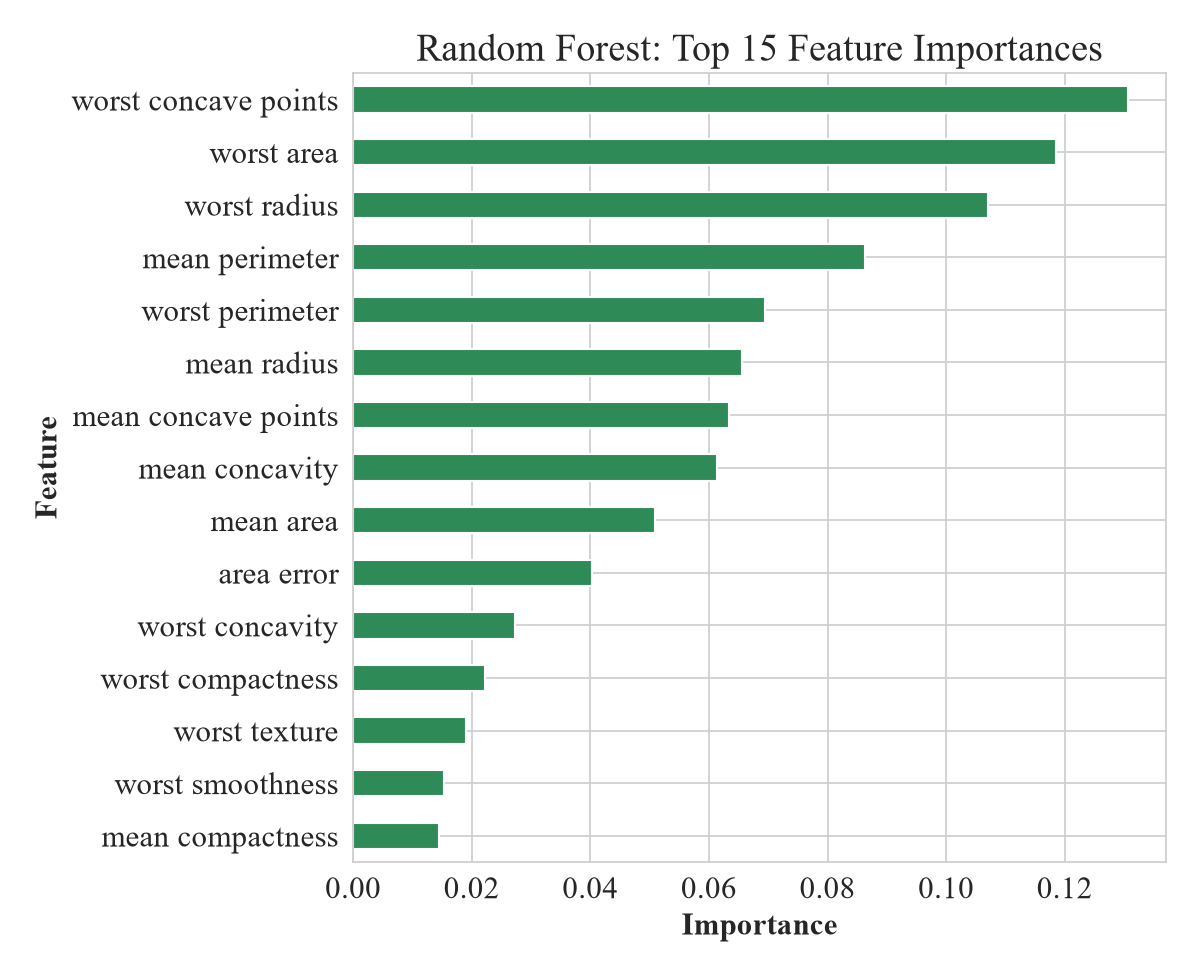
\includegraphics[width=0.75\linewidth]{figures/06_feature_importance.png}
\caption{Random Forest: top 15 feature importances.}
\end{figure}
\textbf{Inference:} \texttt{worst concave points}, \texttt{worst area} and
\texttt{worst radius} are the three most important features, consistent with the EDA
correlation ranking. The importances are spread across several features rather than
dominated by one, reflecting the redundancy among the size-related measurements noted
in Section 4.

\begin{figure}[H]
\centering
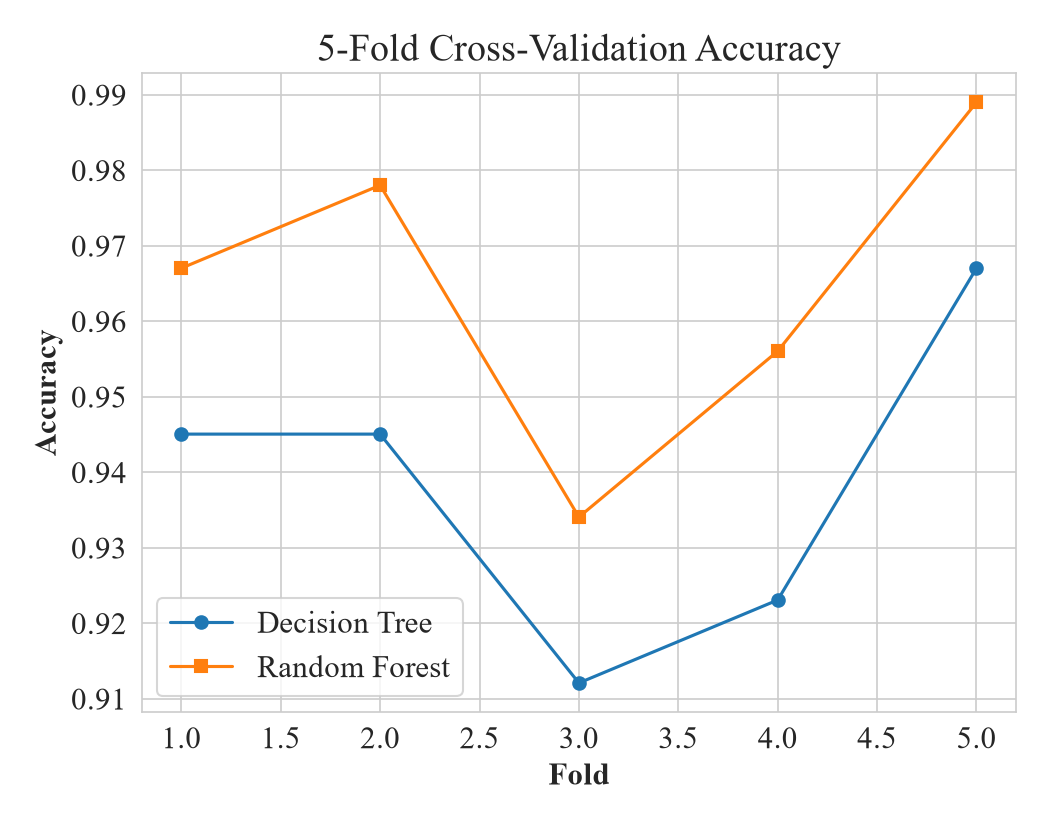
\includegraphics[width=0.7\linewidth]{figures/07_cv_fold_comparison.png}
\caption{5-fold cross-validation accuracy, tuned Decision Tree vs.\ tuned Random
Forest.}
\end{figure}
\textbf{Inference:} The Random Forest outperforms the Decision Tree in every one of the
five folds, by a consistent margin, confirming the average-CV advantage is not an
artifact of how the training set happened to split.

\begin{figure}[H]
\centering
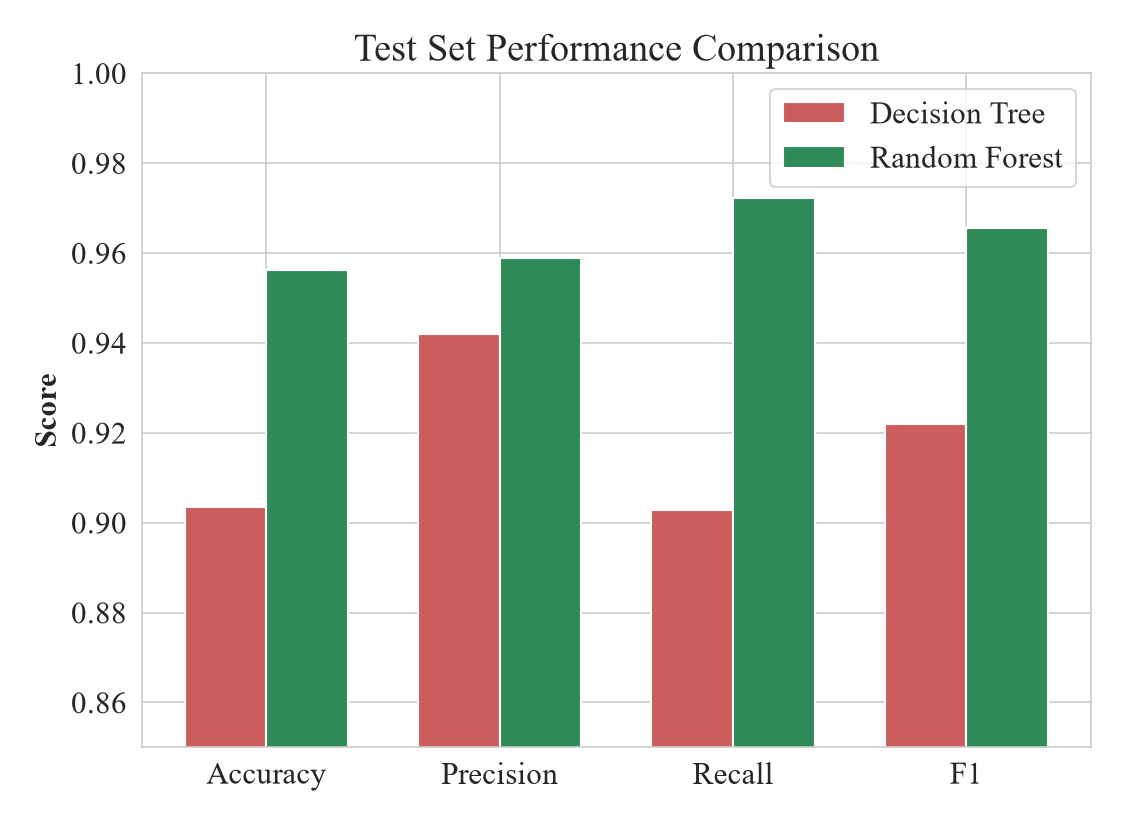
\includegraphics[width=0.75\linewidth]{figures/08_model_comparison.png}
\caption{Test-set accuracy, precision, recall and F1-score, tuned Decision Tree vs.\
tuned Random Forest.}
\end{figure}
\textbf{Inference:} Random Forest leads on every metric, with the largest gap in
recall (0.9722 vs.\ 0.9028), the metric that matters most for avoiding missed
malignant diagnoses.

\begin{figure}[H]
\centering
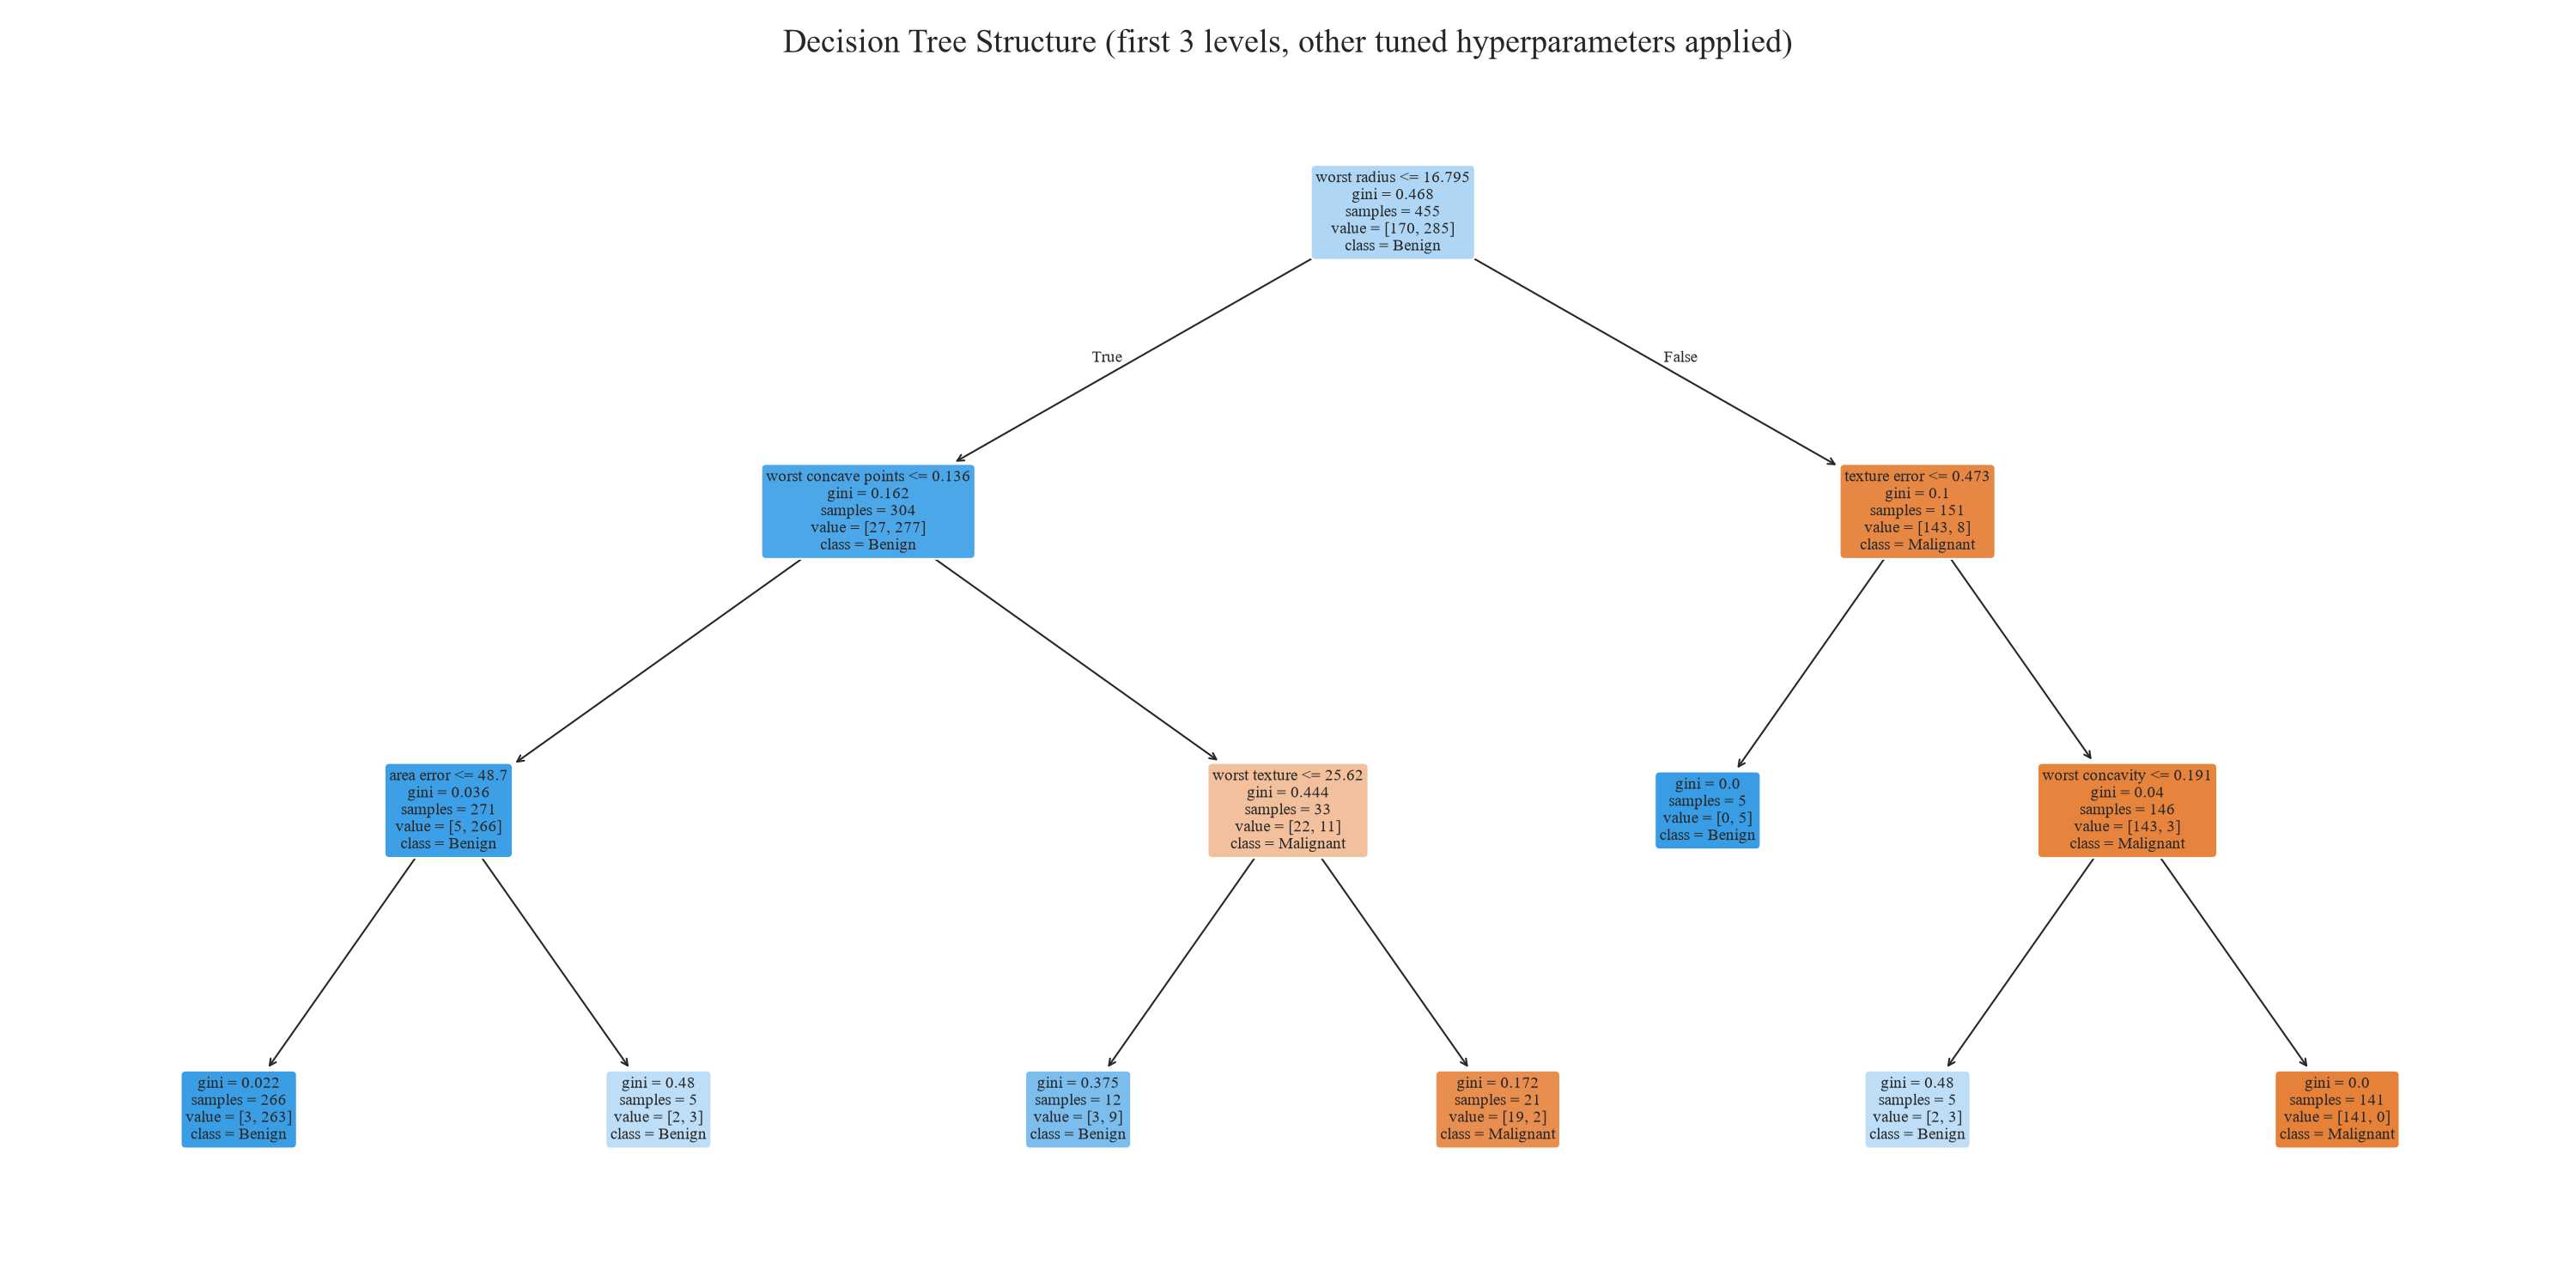
\includegraphics[width=0.95\linewidth]{figures/09_tree_structure.png}
\caption{First three levels of a Decision Tree grown with the tuned criterion,
\texttt{min\_samples\_split} and \texttt{min\_samples\_leaf} (depth capped at 3 purely
for readability; the tuned model used in Results above is not depth-limited to 3).}
\end{figure}
\textbf{Inference:} The root split is on \texttt{worst perimeter} or a closely related
size feature, matching the feature-importance ranking; the tree reaches a mostly-pure
leaf within two or three levels for the more separable regions of the feature space,
which is why a shallow tree already scores well while a much deeper one only adds
overfitting.

\section{Discussion}

\subsection*{Observation Questions}
\textbf{1. How does tree depth affect overfitting in Decision Trees?} Training accuracy
rises monotonically with depth and reaches 1.0000 by \texttt{max\_depth=7} (Figure 1),
since an unrestricted tree keeps splitting until every leaf is pure. Test accuracy,
however, peaks at \texttt{max\_depth=3--4} and then declines to a lower plateau: beyond
that point the extra splits fit noise specific to the training set rather than the
class boundary, which is the definition of overfitting. Depth is the single most
influential Decision Tree hyperparameter for this dataset.

\textbf{2. Which hyperparameter had the greatest impact on performance?} For the
Decision Tree, \texttt{max\_depth} dominates: Table 1 shows CV accuracy varying by
over a full point across depths at fixed criterion, while \texttt{criterion} itself
(gini vs.\ entropy) changes results by well under a point. For the Random Forest,
\texttt{n\_estimators} and \texttt{max\_depth} both matter but with diminishing
returns: moving from 50 to 100 trees improves CV accuracy, but 100 to 200 does not
(Table 2), and depth beyond 10 has no effect once the forest already has enough trees
to average out individual overfitting.

\textbf{3. How does Random Forest improve generalization?} By training many trees on
independent bootstrap samples and restricting each split to a random feature subset,
the individual trees decorrelate from one another. Averaging (via majority vote)
decorrelated, individually high-variance trees cancels out much of that variance while
preserving the low bias of deep trees, which is exactly the pattern seen here: the
Random Forest's cross-validated standard deviation (0.0189) is close to the Decision
Tree's (0.0192), but its mean accuracy is roughly 2.6 points higher across every fold
(Figure 7) and its test-set ROC-AUC is 0.057 higher.

\textbf{4. Did ensemble learning always improve performance? Why or why not?} Not
unconditionally, but it did here on every metric measured. Random Forest improves on
Decision Tree when the individual trees' errors are not perfectly correlated (bagging
plus random feature selection ensures this) and when the dataset has enough signal
that averaging trades a small amount of individual-tree bias for a large reduction in
variance. Ensembling would add little on a dataset so simple that a single shallow
tree already achieves near-ceiling accuracy, and it does not fix a systematic bias
shared by every tree (e.g.\ if the feature set itself lacked signal for a class); its
benefit here comes specifically from reducing the high variance visible in the
Decision Tree's overfitting curve.

\section{Conclusion}
Both models were implemented and tuned via 5-fold cross-validation on the Wisconsin
Diagnostic Breast Cancer dataset. The tuned Decision Tree (\texttt{gini},
\texttt{max\_depth=5}) reached 90.4\% test accuracy and 93.6\% ROC-AUC, while the tuned
Random Forest (100 trees, \texttt{max\_depth=10}, \texttt{max\_features=log2}) reached
95.6\% test accuracy, 96.6\% F1-score and 99.2\% ROC-AUC, outperforming the single tree
on every metric and in every cross-validation fold. The overfitting sweep (Figure 1)
shows why: an unconstrained single tree memorizes the training set, and even a
depth-tuned tree remains sensitive to which 455 samples it happens to see, whereas
bagging and random feature selection let the Random Forest use many such trees without
inheriting any single tree's instability. For a task like malignant-tumour detection,
where missed positives carry a high cost, the Random Forest's substantially higher
recall (0.9722 vs.\ 0.9028) makes it the clearly preferable model here, at the cost of
longer training time and reduced interpretability compared to the single tree's
directly readable decision rules.

\section{References}
\begin{enumerate}
\item Scikit-learn Developers, ``Decision Trees,'' Scikit-learn Documentation.
[Online]. Available: \url{https://scikit-learn.org/stable/modules/tree.html}
\item Scikit-learn Developers, ``Ensemble methods: Random Forests,'' Scikit-learn
Documentation. [Online]. Available:
\url{https://scikit-learn.org/stable/modules/ensemble.html\#random-forests}
\item W. N. Street, W. H. Wolberg, and O. L. Mangasarian, ``Nuclear feature extraction
for breast tumor diagnosis,'' \textit{IS\&T/SPIE International Symposium on Electronic
Imaging}, 1993. Wisconsin Diagnostic Breast Cancer Dataset, UCI Machine Learning
Repository. [Online]. Available: \url{https://archive.ics.uci.edu}
\end{enumerate}

\end{document}
